%!TEX program = xelatex
\documentclass[9pt]{beamer}
    \usepackage[english]{babel}
\usepackage{fancyhdr}        % header footer
\usepackage{graphicx}        % figure
\usepackage{algorithm2e}
\usepackage{booktabs}
\usepackage{xcolor}
\usepackage{bookmark}
\usepackage{xeCJK}
\usepackage{filecontents}
% \usefonttheme{professionalfonts}
\setCJKmainfont[ItalicFont={楷体}, BoldFont={黑体}]{宋体} %  斜体为楷书,加粗黑体,默认宋体
\setbeamertemplate{caption}[numbered]
% \setmainfont{Times New Roman}   %西文默认衬线字体(serif)
% \setsansfont{Arial}   %西文默认无衬线字体(sans serif)
% \setmonofont{Courier New}           %西文默认的等宽字体


    \author{11812214 \textit{任振裕}}
\title{A Joint Learning and Communications Framework
for Federated Learning over Wireless Networks}
\institute{Department of Electrical and Electronic Engineering\\Southern University of Science and Technology}
\date{\today}

% \AtBeginSection[]{
%     \frame{\frametitle{Outline}\tableofcontents[currentsection, 
%     subsectionstyle=show/show/shaded]}
% }




    \usetheme{Simple}
    \useoutertheme{miniframes} %miniframes, tree
\begin{document}
\frame[plain]{\titlepage}
% \frame{\frametitle{Outline}\tableofcontents}
\section{System Model}
\begin{frame}{List of notations}
    \begin{figure}
        \centering
        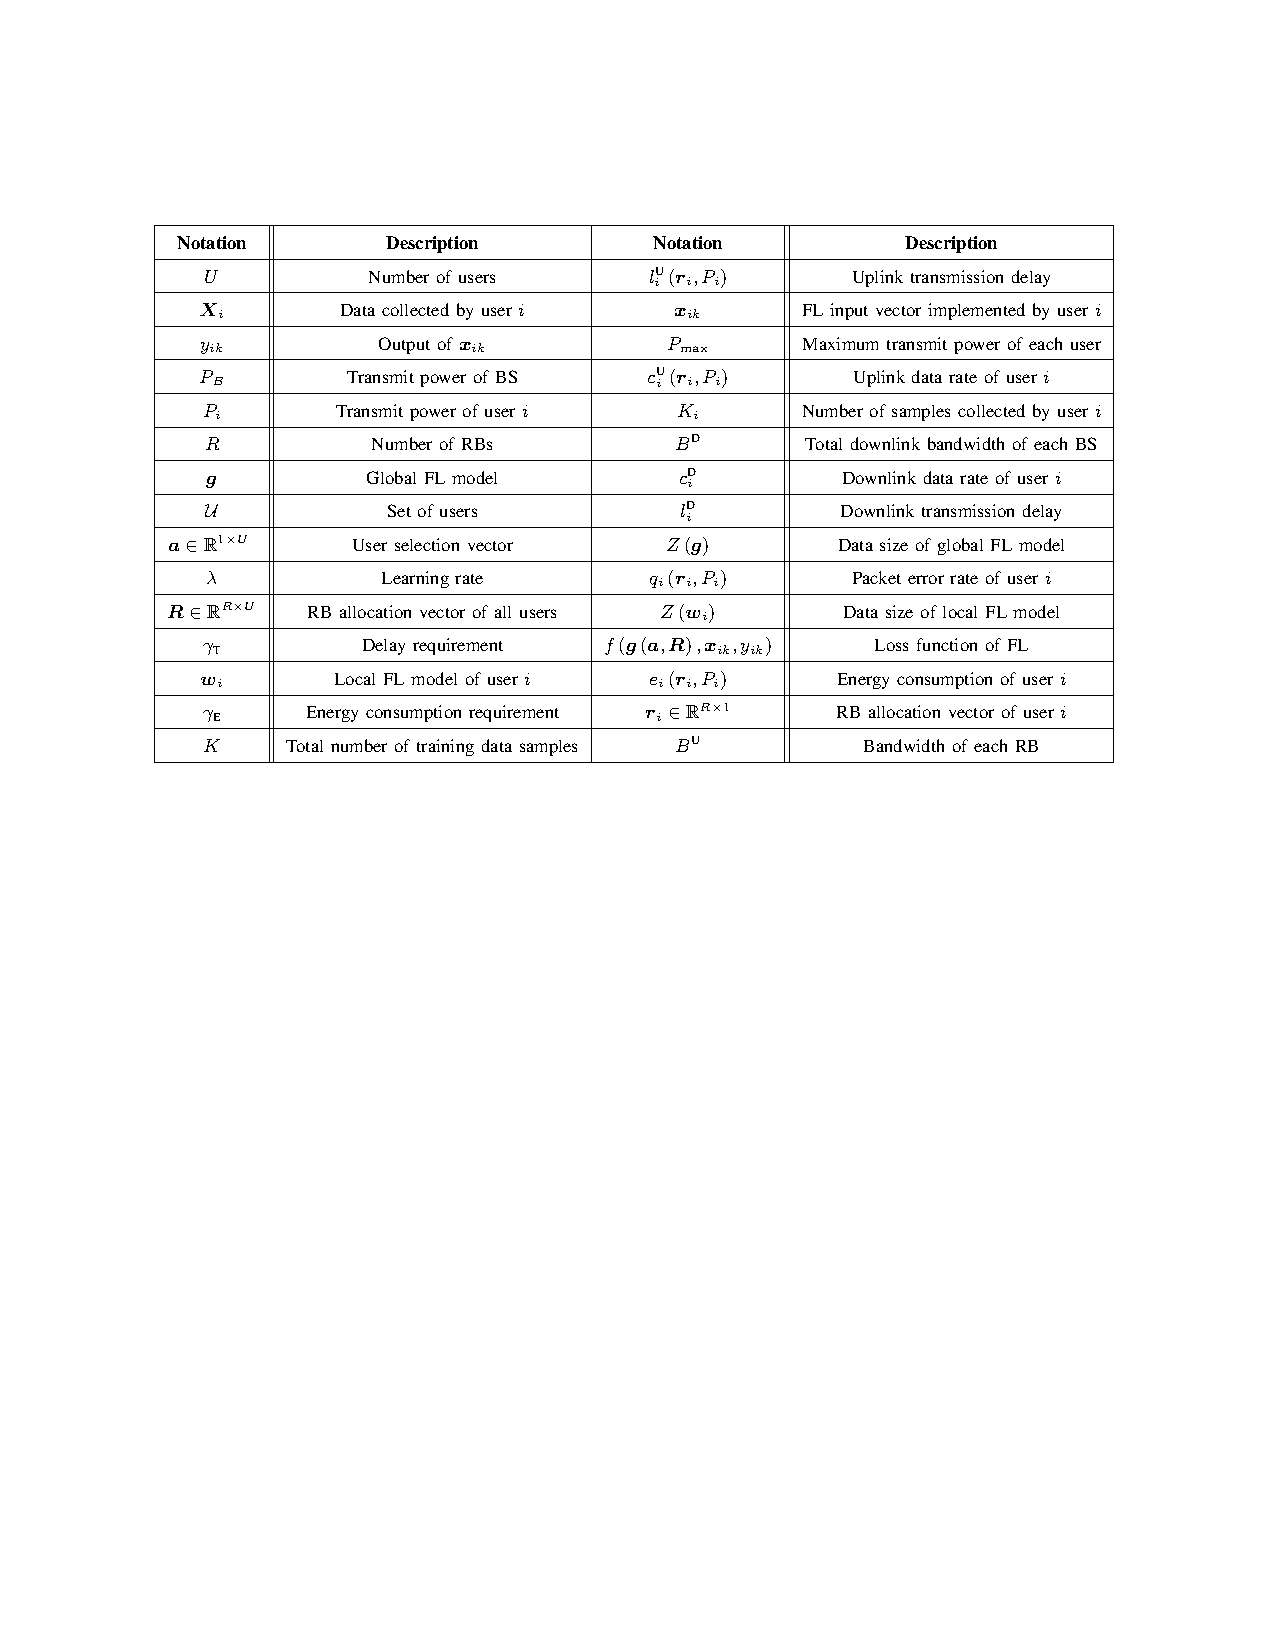
\includegraphics[width=\linewidth]{img/list.pdf}
        \caption{List of notations.} 
    \end{figure}
\end{frame}
\begin{frame}[t]
    \frametitle{Test for citations}
    \begin{itemize}
        \item The first citation.\cite{dl1}
        \item The second citation. \cite{iot1}
        \item Recite the first citation. \cite{dl1}
    \end{itemize}
\end{frame}
\section{Reference}
\begin{frame}[shrink]
    \frametitle{Reference}
    \setbeamertemplate{bibliography item}{\insertbiblabel}
    % \setbeamertemplate{bibliography item}[book]    
    \begin{thebibliography}{100}    
        \bibitem{dl1} Y.~LeCun, Y.~Bengio, and G.~Hinton, ``Deep learning,'' \emph{Nature}, vol. 521, pp. 436--444, May 2015.
        \bibitem{iot1} H.~Li, K.~Ota, and M.~Dong, ``Learning IoT in edge: Deep learning for the Internet of Things with edge computing,'' \emph{IEEE Netw.}, vol.~32, no.~1, pp.~96--101, Feb.~2018.
    \end{thebibliography}    
\end{frame}
\end{document}